\subsection{2(f) Angular acceleration}
\begin{figure}[H]
    \centering
    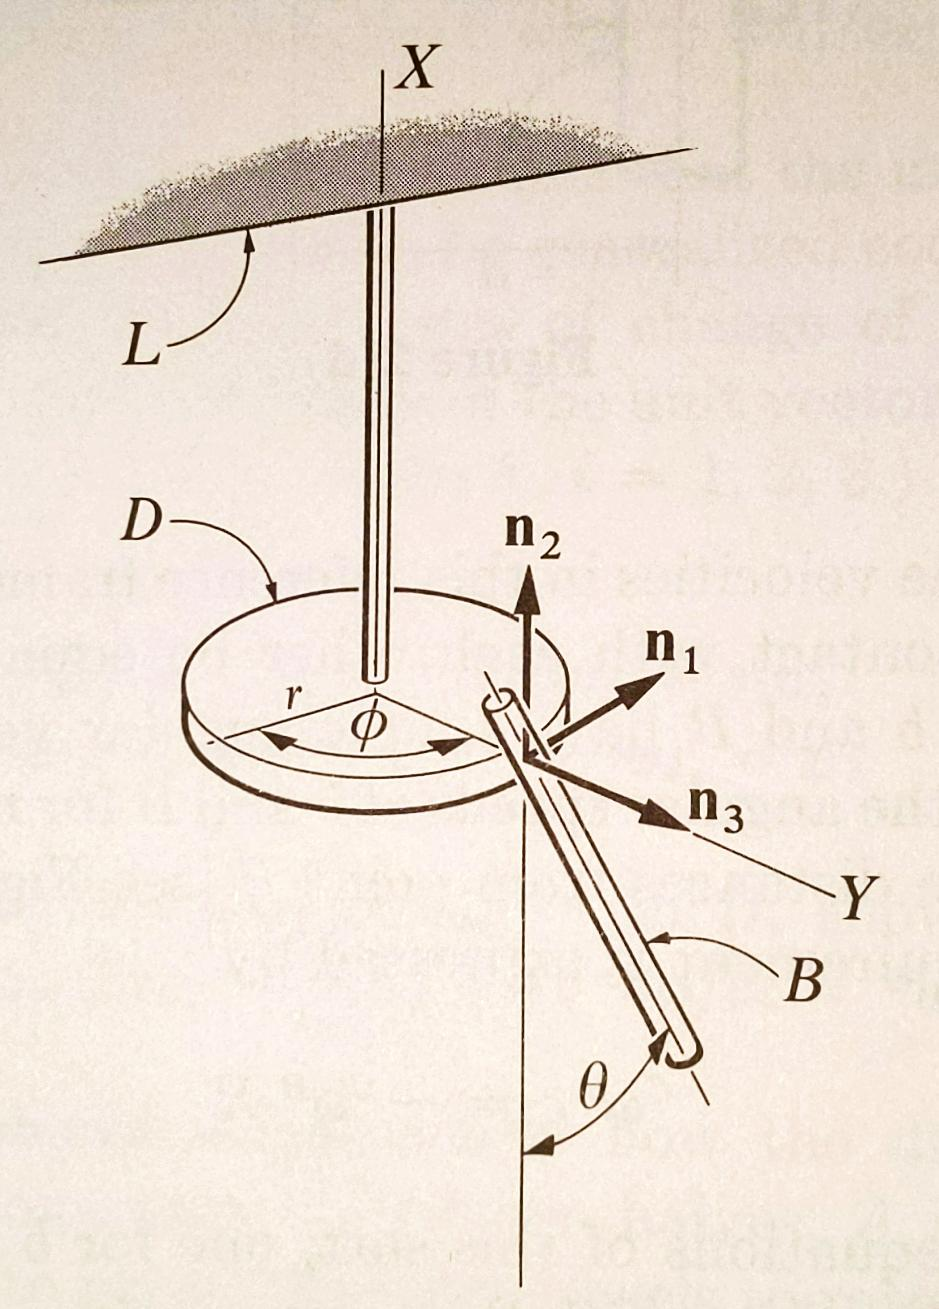
\includegraphics[scale = 0.15]{figs/ProbSet_2/2_f.jpg}
    \caption{}
    \label{2_f}
\end{figure}

\itbf{Sol.}

\begin{align*}
    \lx{^L}{\pmb \omega}{^D} &= \dot \phi \pmb n_2 \qquad and \qquad
    \lx{^L}{\pmb \omega}{^B} = \dot \phi \pmb n_2 + \dot \theta \pmb n_3
\end{align*}

\begin{align*}
    \lx{^L}{\pmb \alpha}{^B} &= \lx{^L}{\frac{d \pmb \omega^B}{d t}}
    %==
    = \lx{^L}{\frac{d}{d t}} \left( \dot \phi \pmb n_2 + \dot \theta \pmb n_3 \right)\\
    %==
    &= \ddot \phi \pmb n_2 + \dot \phi \underbrace{\left( \lx{^L}{\pmb \omega}{^D} \times \pmb n_2 \right)}_{=0} +
    \ddot \theta \pmb n_3 + \dot \theta \underbrace{\left( \lx{^L}{\pmb \omega}{^D} \times \pmb n_3 \right)}_{=\dot \phi n_1}
    %==
    \quad \left[\because \pmb n_1, \pmb n_2, \pmb n_3 \text{ are attached to D (not B)}. \right]\\
    %==
    \implies \lx{^L}{\pmb \alpha}{^B} &= \dot \phi \dot \theta \pmb n_1 + \ddot \phi \pmb n_2 + \ddot \theta \pmb n_2\\
    %===
    \implies& \alpha_1 = \dot \phi \dot \theta, \quad
    \alpha_2 = \ddot \phi, \quad
    \alpha_3 = \ddot \theta
\end{align*}
